\subsection{Caractéristiques pour la représentation et la notation}

\begin{table}[h]
	\centering
	\begin{tabular}{|c|c|c|} \hline
		Pitchs & Instruments \\ \hline
		51 & ride \\
		44 & ch-pf \\
		36 & gc \\
		38 & cc \\
		37 & cross-stick \\ \hline
	\end{tabular}
	\caption{Pitchs et instruments}
	%	\label{tab:exemple}
\end{table}
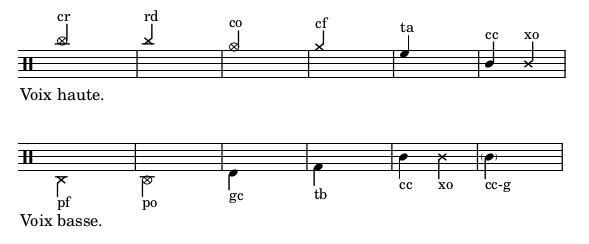
\includegraphics[height=65mm, width=150mm]{images/description_notation/description_notation.png}\\\\
La vélocité sera une donnée importante pour reconnaître les ghosts-notes.\\ Par exemple, pour la caisse-claire, un coup normal (after-beat) monte au dessus de 70 et une ghost-note est autour de 30.
\subsection{Les systèmes}
Créer un ensemble de systèmes :
\begin{itemize}
\item Trouver les systèmes intéressants dans groove ;
\item Compléter avec des systèmes ago personnalisés ;
\item Tout transcrire avec lilypond et en arbres d’analyse syntaxique.
\item Créer les arbres de voix séparées.
\item Créer les arbres de voix séparées simplifiés (rewriting).\\	
\end{itemize}

%preamble:
%
%
%%\usetikzlibrary{backgrounds}
%%\usetikzlibrary{trees}
%
%
%Figure 1:
%
%\begin{figure}
%\centering
%\subfigure
%[$\frac{1}{2} \frac{1}{4} \frac{1}{4}$]
%{
%\begin{tabular}{c}
%%\includegraphics[scale=\scorescale]{images/1a.png}\\
%\begin{tikzpicture} [-,thick]
%\tikzstyle{level 1}=[level distance=7mm,sibling distance=6mm]
%\tikzstyle{level 2}=[level distance=7mm,sibling distance=5mm]
%\node {$\deux$}
%  child { node {$\note$} }
%  child { node {$\deux$}
%    child { node {$\note$} }
%    child { node {$\note$} } };
%\end{tikzpicture}
%\end{tabular}
%\label{fig:subfig1a}}
%%
%\hspace{0.6cm}
%\subfigure
%[$\lbrack \frac{1}{6} \rbrack\, \frac{1}{6}\,
%  \lbrack \frac{1}{6} \rbrack\, \frac{1}{6}\,
%  \lbrack \frac{1}{6} \rbrack\, \frac{1}{6}$]
%{
%\begin{tabular}{c}
%%\includegraphics[scale=\scorescale]{images/1b.png}\\
%\begin{tikzpicture} [-,thick]
%\tikzstyle{level 1}=[level distance=7mm,sibling distance=9mm]
%\tikzstyle{level 2}=[level distance=7mm,sibling distance=5mm]
%\node {$\trois$}
%  child { node {$\deux$}
%    child { node {$\rest$} }
%    child { node {$\note$} } }
%  child { node {$\deux$}
%    child { node {$\rest$} }
%    child { node {$\note$} } }
%  child { node {$\deux$}
%    child { node {$\rest$} }
%    child { node {$\note$} } };
%\end{tikzpicture}
%\end{tabular}
%\label{fig:subfig1b}}
%%
%\hspace{0.6cm}
%\subfigure
%[$\frac{1}{5} \frac{1}{5}
%  \frac{1}{15}\frac{1}{15}\frac{1}{15}
%  \frac{1}{5} \frac{1}{5}$]
%{
%\begin{tabular}{c}
%%\includegraphics[scale=\scorescale]{images/1c.png}\\
%\begin{tikzpicture} [-,thick]
%\tikzstyle{level 1}=[level distance=7mm,sibling distance=5mm]
%\tikzstyle{level 2}=[level distance=7mm,sibling distance=5mm]
%\node {$\cinq$}
%  child { node {$\note$} }
%  child { node {$\note$} }
%  child { node {$\trois$}
%    child { node {$\note$} }
%    child { node {$\note$} }
%    child { node {$\note$} } }
%  child { node {$\note$} }
%  child { node {$\note$} } ;
%\end{tikzpicture}
%\end{tabular}
%\label{fig:subfig1c}}
%%
%\begin{RR}
%\hspace{0.6cm}
%\subfigure
%[$\frac{1}{12} \frac{1}{12} \frac{1}{12} \frac{1}{12} \frac{1}{3}
%\frac{1}{12} \frac{1}{12} \frac{1}{12} \frac{1}{12}$]
%{
%\begin{tabular}{c}
%%\includegraphics[scale=0\scorescale]{images/1d.png}\\
%%\hspace{0.3cm}
%\begin{tikzpicture} [-,thick]
%\tikzstyle{level 1}=[level distance=7mm,sibling distance=9mm]
%\tikzstyle{level 2}=[level distance=6mm,sibling distance=8mm]
%\tikzstyle{level 3}=[level distance=6mm,sibling distance=5mm]
%\node {$\trois$}
%  child { node {$\deux$}
%    child { node {$\deux$}
%      child { node {$\note$} }
%  child { node {$\note$} } }
%    child { node {$\deux$}
%      child { node {$\note$} }
%  child { node {$\note$} } } }
%  child { node {$\note$} }
%  child { node {$\deux$}
%    child { node {$\deux$}
%      child { node {$\note$} }
%  child { node {$\note$} } }
%    child { node {$\deux$}
%      child { node {$\note$} }
%  child { node {$\note$} } } };
%\end{tikzpicture}
%\end{tabular}
%\label{fig:subfig1d}}
%\end{RR}
%\caption{Simple trees of $\T(\Sigmar)$ with their corresponding
%rhythmic notations and values.}
%\label{fig:trees0}
%\end{figure}